\chapter{Implementación del pipeline de generación y normalización}
\label{cap:pipeline}

El Capítulo~\ref{cap:metodologia} presentó la arquitectura general de Open CVN
agrupada en cuatro bloques y detalló, dentro de cada uno, la secuencia de
etapas que los componen. El presente capítulo desciende al último nivel de
concreción antes de la evaluación del sistema: describe cómo se implementa
cada una de esas etapas, qué recibe y qué produce, y qué evidencia concreta
deja el sistema para trazar un campo desde el paquete oficial CVN hasta el
formato Open CVN. El resultado funcional de este pipeline, el propio formato
Open CVN JSON y la herramienta local que lo consume, se presentan en el
Capítulo~\ref{cap:formato_herramienta}.

\section{Generación estructural}
\label{sec:pipeline_generacion_estructural}

La primera etapa del pipeline genera, de forma reproducible, los bindings
Pydantic estructurales a partir de los esquemas XSD oficiales descritos en el
Capítulo~\ref{cap:ecosistema_cvn}. Esta generación se ejecuta mediante
\textit{xsdata} a través de un componente de orquestación propio del
repositorio, que valida los requisitos previos, limpia los directorios de
salida existentes, ejecuta la generación para cada esquema y verifica que el
resultado sea importable antes de darla por completada. La generación se
invoca mediante un comando único que procesa de manera secuencial los siete
paquetes estructurales del sistema: el documento CVN principal, el manual de
especificaciones, el modelo en árbol, las tablas de referencia, los subtipos,
el catálogo de entidades y el tesauro.

El modelo en árbol requiere, además, una configuración específica para evitar
un fallo de generación por dependencias circulares, ya documentado como
limitación en el Capítulo~\ref{cap:ecosistema_cvn}. Esta configuración se
aplica únicamente a ese paquete, en lugar de alterar la configuración general
de generación para el resto de esquemas, de modo que la excepción quede
acotada y explícita.

\section{Normalización de metadatos por código CVN}
\label{sec:pipeline_normalizacion}

Antes de aplicar cualquier interpretación semántica, el sistema necesita una
representación única de cada campo curricular, ya que su información aparece
dispersa entre el manual funcional y el modelo en árbol. La etapa de
normalización resuelve esta dispersión: extrae de forma independiente los
metadatos del manual en XML y las rutas técnicas del modelo en árbol, y a
continuación los unifica en una única entrada por código CVN.

Sobre el paquete oficial descrito en el Capítulo~\ref{cap:ecosistema_cvn}, esta
etapa produce actualmente \textbf{1457} entradas normalizadas. De ellas,
\textbf{27} proceden únicamente del manual funcional y \textbf{1} únicamente
del modelo en árbol; las \textbf{1429} restantes están presentes en ambas
fuentes. El proceso registra, además, \textbf{33} discrepancias entre fuentes,
entre las que se incluye la discrepancia del modelo en árbol ya analizada en
el Capítulo~\ref{cap:ecosistema_cvn}.

El Código~\ref{cod:pipeline_fragmento_normalizado} muestra, de forma reducida
y simplificada, el resultado normalizado del campo de código
\texttt{000.010.000.030}, correspondiente al sexo de la persona, antes de que
la política semántica decida su forma final.

\begin{code}[htbp]
\begin{lstlisting}[language=, basicstyle=\small\ttfamily, breaklines=true]
codigo: "000.010.000.030"
campo_manual: "Sexo"
tabla_referencia_manual: "CVN_SEX_A"
ruta_arbol: "Identification/PersonalIdentification/Gender"
resolucion_referencia:
  estado: resuelto
  fuente: "ReferenceTables.xml"
  evidencia: 2 valores (Hombre, Mujer)
\end{lstlisting}
\caption{Fragmento reducido del metadato normalizado del campo de sexo.}
\label{cod:pipeline_fragmento_normalizado}
\end{code}

\section{Resolución de referencias auxiliares}
\label{sec:pipeline_resolucion_auxiliar}

Una parte considerable de los campos del manual remite a una tabla de
valores controlados en lugar de admitir texto libre. La etapa de resolución
de referencias auxiliares comprueba, para cada campo con una tabla asociada,
si dicha tabla puede resolverse contra las tablas de referencia, los
subtipos, el catálogo de entidades o el tesauro descritos en el
Capítulo~\ref{cap:ecosistema_cvn}, y registra el resultado como evidencia
explícita adjunta al metadato normalizado.

De las 1457 entradas normalizadas, \textbf{557} incluyen una tabla de
referencia en el manual y, por tanto, pasan por esta etapa; las \textbf{900}
restantes corresponden a campos de texto, fecha o número sin tabla asociada.
La Tabla~\ref{tab:pipeline_resolucion_auxiliar} desglosa esas 557 entradas
según el tipo de evidencia de resolución obtenida.

\begin{table}[htbp]
  \centering
  \small
  \renewcommand{\arraystretch}{1.2}
  \begin{tabular}{p{0.5\textwidth} r}
    \hline
    \textbf{Tipo de evidencia de resolución} & \textbf{Entradas} \\
    \hline
    Tabla compacta de tipo enumeración & 258 \\
    Clasificación temática jerárquica & 125 \\
    Registro de entidad de un paquete auxiliar & 93 \\
    Clasificación de ámbito o alcance & 16 \\
    Tesauro o vocabulario de un paquete auxiliar & 27 \\
    Familia controlada respaldada por subtipos & 20 \\
    Tabla de tipo identificador & 11 \\
    Escala o medida compacta & 6 \\
    Referencia no resuelta & 1 \\
    \hline
    \textbf{Total con tabla de referencia} & \textbf{557} \\
    \hline
  \end{tabular}
  \caption{Resultado de la resolución de referencias auxiliares sobre las entradas normalizadas con tabla asociada.}
  \label{tab:pipeline_resolucion_auxiliar}
\end{table}

Estos resultados confirman con evidencia concreta dos afirmaciones ya
adelantadas en el Capítulo~\ref{cap:ecosistema_cvn}. Por un lado, únicamente
una entrada permanece sin resolver dentro del paquete analizado: el campo de
código \texttt{060.010.000.030} (\emph{Fuente de índice H}), cuya tabla
declarada en el manual no tiene equivalente directo en el resto del paquete.
Por otro lado, la tabla del campo de sexo (\texttt{000.010.000.030}) se
resuelve contra las tablas de referencia con solo dos valores posibles, sin
jerarquía, delegados ni entradas duplicadas, lo que constituye la evidencia
que permite tratarla como una enumeración cerrada en la etapa siguiente.

\section{Política semántica}
\label{sec:pipeline_politica_semantica}

Los esquemas XSD oficiales solo indican cómo se serializa un campo, no cómo
debe representarse en un modelo de dominio: un mismo tipo XSD genérico puede
esconder tanto un texto libre como un conjunto cerrado de valores
controlados, y una tabla auxiliar puede ser tan pequeña como la del campo de
sexo o tan abierta como un catálogo institucional en crecimiento. El
Capítulo~\ref{cap:ecosistema_cvn} ya identificó esta ambigüedad como una
limitación del paquete oficial. La política semántica es la etapa que la
resuelve: toma los metadatos normalizados y, cuando existe, la evidencia de
resolución de la etapa anterior, y decide de forma explícita y trazable qué
forma debe adoptar cada campo en el modelo de dominio, sin dejar nunca esa
decisión implícita en el tipo XSD de origen.

\subsection{Formas semánticas reconocidas}
\label{sec:pipeline_politica_formas}

La política reconoce nueve formas semánticas base. La Tabla~\ref{tab:pipeline_formas_semanticas}
las describe junto con un ejemplo real tomado del paquete oficial CVN.

\begin{table}[htbp]
  \centering
  \small
  \renewcommand{\arraystretch}{1.2}
  \begin{tabular}{p{0.22\textwidth} p{0.4\textwidth} p{0.3\textwidth}}
    \hline
    \textbf{Forma semántica} & \textbf{Qué representa} & \textbf{Ejemplo} \\
    \hline
    Texto & Cadena libre sin tabla de valores asociada & Título de una publicación \\
    Fecha & Valor temporal, completo o parcial & Fecha de inicio de un contrato \\
    Número & Valor numérico & Número de horas impartidas \\
    Enumeración cerrada & Tabla auxiliar con evidencia suficiente para tratarse como un conjunto fijo de valores & Sexo (tabla \texttt{CVN\_SEX\_A}) \\
    Catálogo abierto & Tabla auxiliar cuya evidencia impide tratarla como cerrada & Tipo de entidad (tabla \texttt{CVN\_ENTITY\_TYPE}) \\
    Referencia a entidad & Remite al catálogo de instituciones y organizaciones del paquete auxiliar & Entidad que participa en un proyecto \\
    Término de tesauro & Remite al vocabulario jerárquico de materias del paquete auxiliar & Palabra clave de una publicación \\
    Valor respaldado por subtipo & Remite a la codificación de subtipos derivada de una tabla auxiliar & Propiedad industrial (tabla \texttt{CVN\_KNOW\_A}) \\
    Referencia no resuelta & La tabla declarada en el manual no tiene equivalente localizable en el resto del paquete & Fuente de índice H (tabla \texttt{CVN\_AGENCY\_C}) \\
    \hline
  \end{tabular}
  \caption{Formas semánticas reconocidas por la política semántica.}
  \label{tab:pipeline_formas_semanticas}
\end{table}

Las tres primeras formas se asignan directamente a los campos que no
declaran ninguna tabla de referencia en el manual, es decir, a las 900
entradas identificadas en el apartado anterior. Las seis formas restantes se
deciden a partir de la evidencia de resolución obtenida para las 557 entradas
que sí declaran una tabla, y son las que exigen una regla de decisión más
cuidadosa.

\subsection{Enumeración cerrada frente a catálogo abierto}
\label{sec:pipeline_politica_enum}

La distinción más delicada de la política es la que separa una enumeración
cerrada de un catálogo abierto, porque ambas parten del mismo punto: una
tabla compacta de tipo enumeración, ya identificada en la
Tabla~\ref{tab:pipeline_resolucion_auxiliar}. La política no decide esta
distinción por el número de valores de la tabla, sino por su comportamiento:
declara ineligible para enumeración cerrada cualquier tabla que presente
jerarquía interna o un valor delegado, es decir, un valor que remite a un
texto libre adicional en lugar de cerrar el conjunto de opciones.

Los dos ejemplos ya utilizados en este capítulo ilustran por qué el tamaño
por sí solo no basta. La tabla del campo de sexo (\texttt{CVN\_SEX\_A})
contiene únicamente 2 valores, sin jerarquía ni delegados, y se declara
elegible como enumeración cerrada. La tabla del campo de tipo de entidad
(\texttt{CVN\_ENTITY\_TYPE}) contiene 17 valores, un tamaño que podría
parecer igualmente manejable, pero incluye un valor delegado de tipo
``Organismo, Otros'' y una etiqueta repetida; por esa evidencia, la política
la declara ineligible y la trata como catálogo abierto. Tratar
\texttt{CVN\_ENTITY\_TYPE} como una enumeración cerrada habría obligado a
elegir, para cualquier entidad que no encajase en las 17 categorías
previstas, entre forzar un valor incorrecto o rechazar el dato; el catálogo
abierto evita ambos problemas conservando el valor literal declarado.

\subsection{Presencia, nomenclatura y traza}
\label{sec:pipeline_politica_presencia}

Además de la forma semántica, la política determina si un campo es
obligatorio u opcional y si admite un único valor o varios, y propone un
nombre de dominio en español derivado del nombre que el campo recibe en el
manual: el campo manual ``Sexo'' se convierte, por ejemplo, en el atributo de
dominio \texttt{sexo}, obligatorio y de valor único. Cada una de estas
decisiones queda acompañada de una traza explícita que identifica la regla
aplicada y su nivel de confianza, de modo que cualquier campo del modelo de
dominio pueda justificarse frente a la fuente CVN concreta de la que
procede, sin depender de inspeccionar de nuevo el XML o el XSD originales.

\section{Generación de modelos de dominio y del modelo conceptual}
\label{sec:pipeline_modelos_dominio}

La política semántica decide, campo a campo, cómo debe representarse cada
dato; esta etapa aplica esa decisión dos veces, con dos propósitos distintos
que conviene no confundir.

En primer lugar, el generador de modelos de dominio traduce la política
semántica completa en clases Pydantic ejecutables: un artefacto de
implementación, en Python, que ya no expone la estructura XML subyacente. La
generación canónica produce actualmente \textbf{105} archivos: 101 módulos
correspondientes a otros tantos conceptos curriculares del modelo en árbol,
un módulo para los campos presentes únicamente en el manual, otro para los
nodos del árbol sin código de manual asociado, y un módulo de enumeraciones
con las \textbf{13} tablas que la política semántica clasificó como
enumeración cerrada.

En segundo lugar, el extractor conceptual reagrupa esa misma información,
sin volver a inspeccionar el XML o el XSD, en una representación ya
independiente de Python: áreas curriculares, entidades conceptuales,
atributos y vocabularios. Esta segunda representación es necesaria porque los
modelos de dominio siguen atados a un lenguaje de implementación concreto,
mientras que los diagramas UML y el formato Open CVN JSON necesitan una
descripción agnóstica de la que partir. Siguiendo el ejemplo de este
capítulo, el campo de sexo se integra así en la entidad conceptual
\texttt{Person} del área \texttt{identity}, la misma agrupación en la que
reaparece su definición final en la Sección~\ref{sec:pipeline_json_schema}.

\section{Generación de JSON Schema y trazabilidad}
\label{sec:pipeline_json_schema}

La última etapa del pipeline genera, a partir del inventario conceptual, el
artefacto JSON Schema que valida de forma declarativa el formato Open CVN
JSON descrito en el Capítulo~\ref{cap:formato_herramienta}. El esquema generado declara la versión Draft
2020-12 y contiene actualmente \textbf{182} definiciones, de las cuales
\textbf{74} corresponden a vocabularios controlados y el resto a entidades
conceptuales y componentes de valor compartidos.

Cada definición generada conserva, junto a su forma de validación, un
conjunto de anotaciones no validantes con el prefijo \texttt{x-open-cvn-},
que registran el código CVN de origen, la referencia de tabla utilizada, la
elegibilidad de enumeración decidida y las rutas XML asociadas. Estas
anotaciones son el mecanismo concreto de trazabilidad que conecta cada
definición del formato Open CVN con la fuente CVN de la que procede. La
Figura~\ref{fig:pipeline_trazabilidad} recorre esta cadena completa para el
campo de sexo ya utilizado como ejemplo en este capítulo, desde sus dos
fuentes en el paquete oficial hasta su definición final en el esquema Open
CVN.

\begin{figure}[htbp]
  \centering
  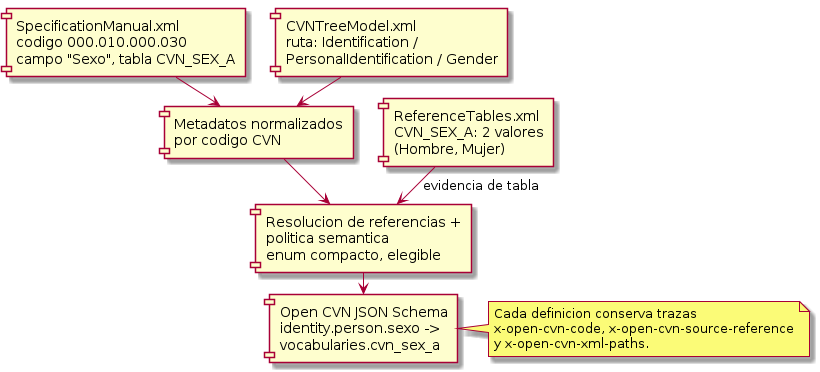
\includegraphics[width=0.8\textwidth]{figs/open_cvn_field_traceability.png}
  \caption{Trazabilidad de un campo desde el paquete oficial CVN hasta el esquema Open CVN JSON.}
  \label{fig:pipeline_trazabilidad}
\end{figure}

Esta misma cadena de trazabilidad se aplica, sin excepción, a cualquier campo
que atraviese el pipeline, incluidos aquellos que terminan en una referencia
no resuelta: en esos casos, la anotación conserva la tabla original citada
por el manual y un mensaje de diagnóstico explícito, en lugar de omitir el
campo o de asignarle una forma semántica no justificada.

\section{Síntesis de las etapas del pipeline}
\label{sec:pipeline_sintesis}

La Tabla~\ref{tab:pipeline_etapas} resume las etapas descritas en este
capítulo, indicando para cada una su entrada, su salida y el módulo del
repositorio que la implementa, ya presentado con mayor detalle arquitectónico
en el Capítulo~\ref{cap:metodologia}.

\begin{table}[htbp]
  \centering
  \small
  \renewcommand{\arraystretch}{1.2}
  \begin{tabular}{p{0.17\textwidth} p{0.24\textwidth} p{0.24\textwidth} p{0.20\textwidth}}
    \hline
    \textbf{Etapa} & \textbf{Entrada} & \textbf{Salida} & \textbf{Módulo} \\
    \hline
    Generación estructural & Esquemas XSD oficiales & Bindings Pydantic estructurales & \path{src/generated/} \\
    Normalización & Manual funcional y modelo en árbol & Metadatos unificados por código CVN & \path{src/cvn_codegen/} \\
    Resolución de referencias auxiliares & Metadatos normalizados y familias auxiliares & Evidencia de resolución por campo & \path{src/cvn_codegen/} \\
    Política semántica & Metadatos normalizados y resueltos & Forma semántica trazable por campo & \path{src/cvn_codegen/} \\
    Generación de modelos de dominio & Política semántica & Modelos de dominio Pydantic & \path{src/models/cvn/} \\
    Extracción del modelo conceptual & Modelos de dominio y decisiones previas & Inventario conceptual agnóstico & \path{src/cvn_codegen/} \\
    Generación de diagramas & Inventario conceptual & Diagramas UML en PlantUML & \path{src/cvn_codegen/} \\
    Generación de JSON Schema & Inventario conceptual & Esquema Open CVN JSON & \path{schemas/} \\
    \hline
  \end{tabular}
  \caption{Etapas del pipeline de generación y normalización, entrada, salida y módulo responsable.}
  \label{tab:pipeline_etapas}
\end{table}

En conjunto, este pipeline demuestra que la trazabilidad hacia CVN exigida en
el Capítulo~\ref{cap:ecosistema_cvn} no es una declaración de intenciones,
sino una propiedad verificable de cada campo generado. El
Capítulo~\ref{cap:formato_herramienta} retoma el resultado final de este pipeline, el formato Open CVN
JSON, y describe su validación, su importación y la herramienta local que lo
utiliza.
